%!TEX root = ../thesis.tex

% \pagebreak[4]
% \hspace*{1cm}
% \pagebreak[4]
% \hspace*{1cm}
% \pagebreak[4]

\chapter{Mélange d'outils}

\graphicspath{ {Chapter3/Chapter3Figs/PNG/}
  {Chapter3/Chapter3Figs/PDF/} {Chapter3/Chapter3Figs/} }

Nous avons vu dans le premier chapitre que les outils de déformation avaient
différentes caractéristiques. Celles-ci influent sur l'aspect de la déformation
engendrée par le déplacement de points de contrôle, ainsi que sur la facilité de
déformation de l'objet. Une modification grossière de l'apparence globale de
l'objet sera plus facile à réaliser avec un outil permettant de réaliser des
déformations globale ayant une faible résolution. A l'inverse, une modification
fine un ensemble de points précis de l'objet nécessitera l'utilisation d'un
outil de déformation ayant une zone d'influence limitée et une résolution
élevée. On se demande alors comment combiner différents outils associé à un même
objet, de façon à ce que la déformation soit visuellement lisse. Autrement dit,
on recherche une méthode de combinaison de plusieurs outils qui conserve les
propriétés de continuité des outils combinés.

\section{Etat de l'art}

On peut citer \cite{JBPS11} comme étant les premiers à proposer une méthode
permettant de mélanger des outils de déformation de différentes dimensions.
C'est sur celui-ci que nous avons commencé à travailler car les résultats nous
semblaient proches de ce que nous souhaitons réaliser. Une lecture approfondie
de l'article nous a fait comprendre que la méthode n'était pas celle que nous
souhaitions. En effet, s'ils semblent s'appuyer sur des outils ayant des
dimensions différentes en fonction des zones à déformer, la gestion interne
repose uniquement sur des déformations à base de points. L'aspect
"multidimensionnel" est donc uniquement présent comme une contrainte
supplémentaire lors du calcul des coordonnées. Par exemple pour des sommets
reliés par une arête les auteurs définissent que les coordonnées évoluent de
façon linéaire le long de cette arête. De plus, pour évaluer l'influence d'un
point de contrôle sur l'espace, la technique proposée se base sur une méthode de
diffusion (nécessitant donc une discrétisation de l'espace). Or un des critères
essentiels de notre travail est la minimisation des temps de calcul, c'est
pourquoi nous avons décidé de pas continuer à étudier cette technique et à nous
intéresser à un autre travail du domaine.

\cite{GPCP13} quant à eux, proposent une méthode permettant le mélange
d'outils de même dimension, en s'intéressant particulièrement aux cas des
déformations à base de cage. Nous nous sommes intéressés à cet article de par sa
récente publication, sa proximité avec \cite{Hur12}, un travail réalisé par un
étudiant en Master ISI en 2012, et de l'utilisation de cages de déformation, le
modèle semblant le plus utilisé ces dernières années parmi les outils à base de
surfaces. L'idée est de réaliser un pavage de différentes cages collées ensemble
le long de leurs arêtes sur tout l'espace à déformer et de considérer la
position d'un point de l'espace, et pas seulement par rapport à sa cage
\textit{propre} (à comprendre la cage englobant le point de l'espace) mais aussi
par rapport aux cages adjacentes à celle-ci. Cette technique permet de localiser
la déformation engendrée par un sommet d'une cage sur la zone couverte par sa
cage propre et l'ensemble des cages incidentes à celle-ci. Cette méthode impose
de placer des cages sur l'ensemble de l'objet, peu importe la déformation à
appliquer dessus. Les cages créées doivent être collées ensembles le long de
leurs arêtes pour que la méthode fonctionne, et cette contrainte alourdit les
traitements à effectuer, du fait des nombreux cas spécifiques que la méthode
doit traiter. Cette méthode repose en interne sur une discrétisation de l'espace
par l'utilisation de coordonnées harmoniques, or la minimisation du temps de
calcul est une de nos priorités.

Etant donné que les solutions existantes ne correspondaient pas vraiment à ce
que nous souhaitions, nous avons décidé de travailler sur une autre approche.
Cette méthode n'a pas pour but de remplacer celles existantes, mais d'apporter
une autre vision au niveau des mélanges d'outils de déformation possibles.

\section{Méthode proposée}

Nous nous sommes concentrés sur des déformations à base de cage, certaines idées
de \cite{GPCP13} nous ont semblé intéressantes, et nous avons décidé de nous en
inspirer. Notre contribution se décompose en 2 parties :

\begin{enumerate}

\item Modifier la zone d'influence des déformations à base de cages

\item Combiner les effets des déformations appliquées par les différentes cages

\end{enumerate}

\subsection{Modification de la zone d'influence des déformations}

Une première solution serait de définir des coordonnées uniquement pour les
points de l'espace à l'intérieur de la cage et de ne pas tenir compte des
points à l'extérieur. Cela amène des problèmes de continuité au niveau des
bords de la cage. Visuellement, la transition entre l'intérieur et l'extérieur
de la cage est brusque et la déformation n'est pas lisse (Figure \ref{MELVI}).

\begin{figure}[ht]
  \begin{center}
    \scalebox{0.2}
    {
      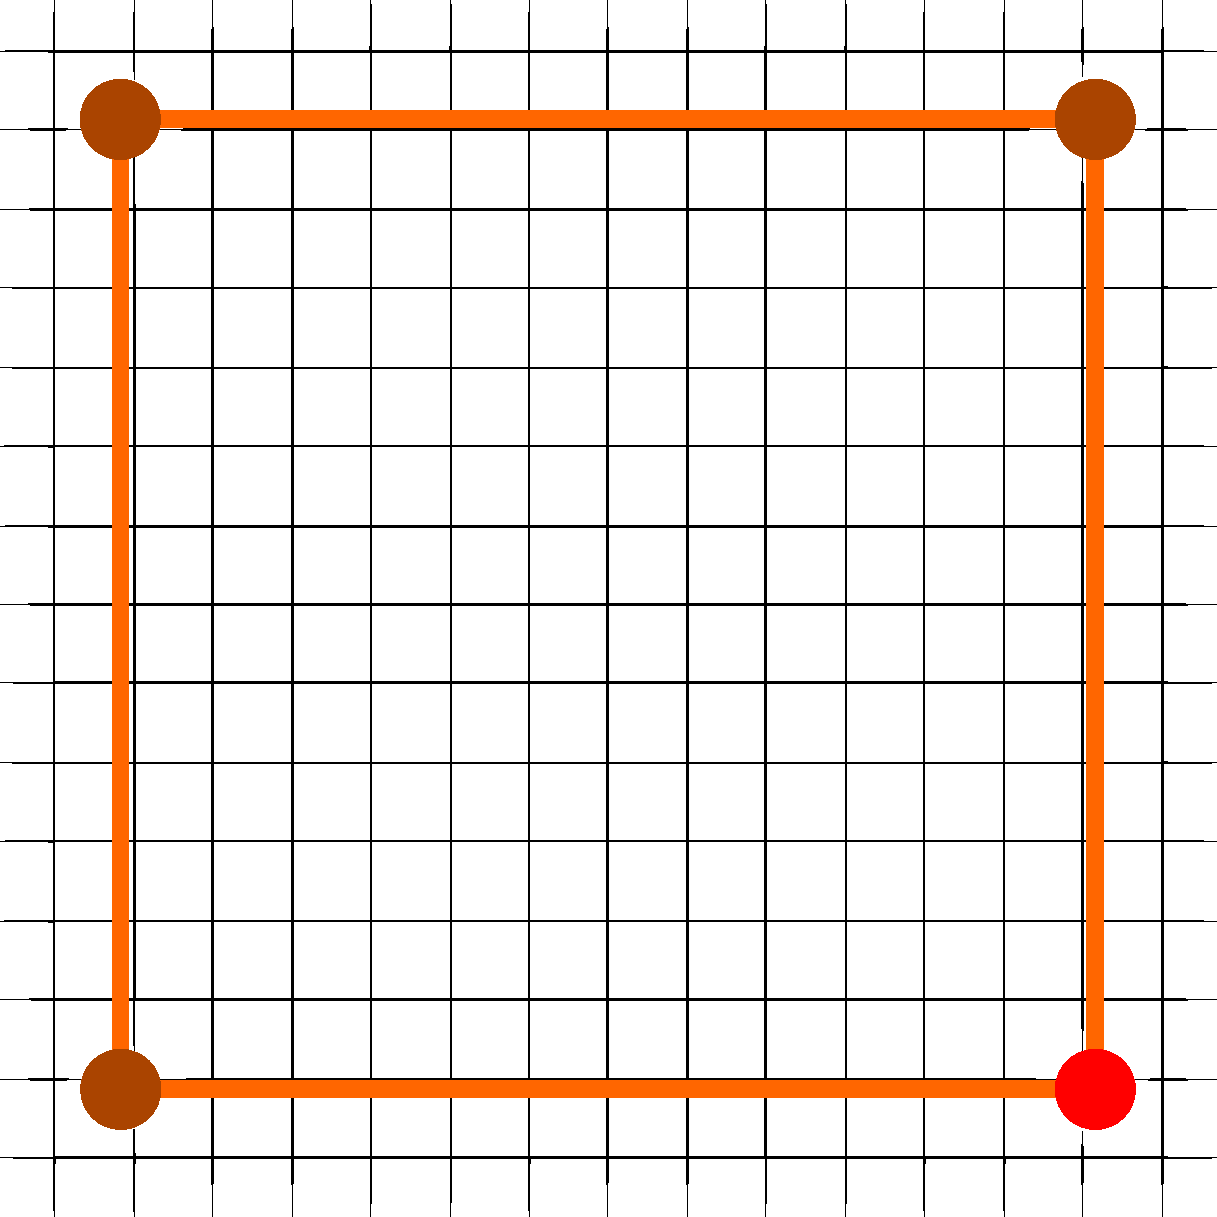
\includegraphics{Deformation-Interieur-1Sommet-Avant}
      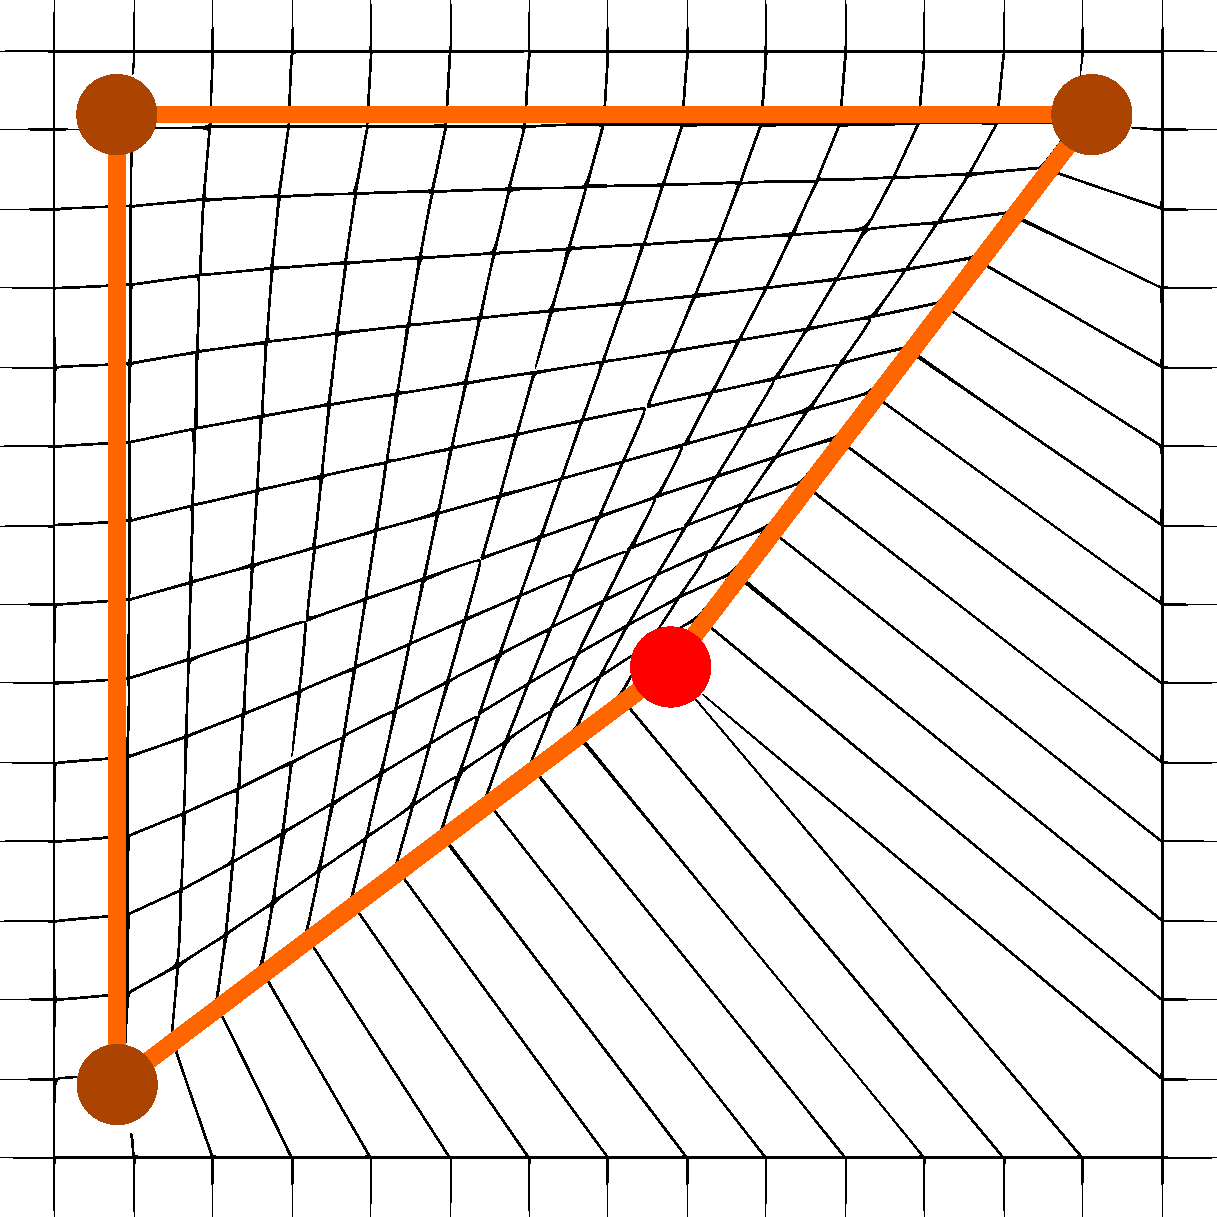
\includegraphics{Deformation-Interieur-1Sommet-Apres}
    }

    \caption{Visualisation des problèmes de continuité lorsque seuls les
points à l'intérieur sont déformés. Le bord de la cage est représenté en bleu.
Le sommet en rouge représente le sommet déplacé. A gauche le modèle avant
déformation, à droite le même modèle après déformation.}

    \label{MELVI}
  \end{center}
\end{figure}

Une autre solution serait de définir des coordonnées pour les points de
l'espace à la fois à l'intérieur et à l'extérieur de la cage. Certaines
méthodes de calcul des coordonnées (comme les MVC ou les GC) sont définies sur
$\mathbb{R}^2$, il serait donc possible de définir des coordonnées pour tous
les points de l'espace. Le problème vient du fait que la fonction résultant du
calcul des coordonnées n'est pas dérivable sur tout le domaine. Plus
précisément, la fonction est $C^{\infty}$ partout, mais elle n'est que $C^0$
au niveau des sommets de la cage. On ne peut donc pas utiliser les coordonnées
existantes telles quelles.

Mais pourquoi les déformations à base de cage ne pourraient pas avoir le même
comportement que les déformations à base de points? On aurait une cage qui
déformerait à la fois les points de l'espace en son intérieur et à
l'extérieur.  Son influence diminuerait progressivement au fur et à mesure que
les points de l'espace soient éloignés du centre de la cage, jusqu'à n'avoir
plus aucune influence au delà d'un certain rayon.

Notre objectif est donc d'obtenir une fonction de déformation, définie par une
cage, qui soit au moins $C^1$ partout et dont l'influence soit limitée à une
certaine zone.

On pourrait se pencher sur la mise en place d'une nouvelle méthode de calcul
de coordonnées ayant les propriétés que nous souhaitons, mais la difficulté de
ce travail en fait un sujet de recherche en soi. Nous nous sommes plutôt
intéressés à la réutilisation des méthodes de calcul existantes, afin de
pouvoir se servir des qualités de ces méthodes.

\subsubsection{Idée}

Considérons deux cages au lieu d'une. Nous appelerons \textit{cage de
contrôle} la cage avec laquelle l'utilisateur va interagir pour réaliser les
déformations. Nous appelerons \textit{cage d'influence} la cage qui va définir
la zone d'influence, zone qui délimite les points de l'espace qui seront sous
l'influence de la cage de contrôle. La cage d'influence correspond à une
version mise à l'échelle de la cage de contrôle, de façon à ce que la cage
d'influence englobe totalement la cage de contrôle (Figure \ref{MELDou}).

\begin{figure}[ht]
  \begin{center}
    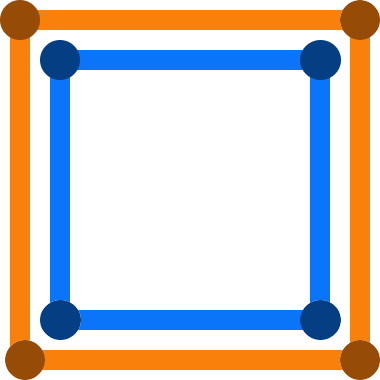
\includegraphics[scale=0.3]{DoubleCage}
    \caption{Disposition des deux cages. En bleu la cage de contrôle, en orange
    la cage d'influence.}
    \label{MELDou}
  \end{center}
\end{figure}

Au lieu de voir la zone d'influence comme l'extérieur de la cage de contrôle,
nous avons décidé de la voir comme l'intérieur de la cage d'influence. Il se
trouve que les coordonnées MVC sont $C^{\infty}$ à l'intérieur de la cage
d'influence (par définition), les déformations qui ont lieu à l'intérieur de
celle-ci sont donc visuellement lisses. On introduit donc ici une notion de
hiérarchie de déformation, où la modification de la position des sommets de la
cage de contrôle va modifier la position des sommets de la cage d'influence,
qui elle-même va modifier l'espace contenu en son intérieur, grâce aux
méthodes de calcul de coordonnées existantes (MVC, HC, GC). \\

\subsubsection{Hiérarchie de la déformation}

Il faut maintenant établir un lien entre les deux cages, afin que la
modification de la position des sommets de la cage de contrôle affecte la
position des sommets de la cage d'influence.

Une première idée serait d'utiliser des coordonnées barycentriques
généralisées pour définir la position de chacun des sommets de la cage
d'influence comme une combinaison linéaire pondérée des positions des sommets
de la cage de contrôle. Cette technique pose un problème quant à la localité
de la déformation. Car même si  la position de tous les points de l'espace
appartenant à la zone d'influence de la cage est modifiée à la modification de
la position d'un seul sommet de la cage, on souhaiterait que les points les
plus éloignés du sommet modifié soient le moins affecté par la déformation.

A la place, on peut définir que chaque sommet de la cage d'influence est lié à
un seul sommet de la cage de contrôle. Etant donné que l'on construit la cage
d'influence comme une version mise à l'échelle de la cage de contrôle, on peut
facilement lier les sommets de la cage de contrôle à leur homologues "mis à
l'échelle" de la cage d'influence. Ainsi, quand on modifie la position d'un
sommet de la cage de contrôle, un seul sommet de la cage d'influence est
déplacé.

On définit donc le lien établit par un vecteur $\overrightarrow{v}$
représentant la différence de position entre un sommet de la cage d'influence
$v_{inf}$ par rapport au sommet de la cage de contrôle $v_{con}$ auquel il est
associé :

\begin{displaymath}
  \overrightarrow{v} = v_{inf}-v_{con}
\end{displaymath}

\begin{figure}[ht]
\begin{center}
  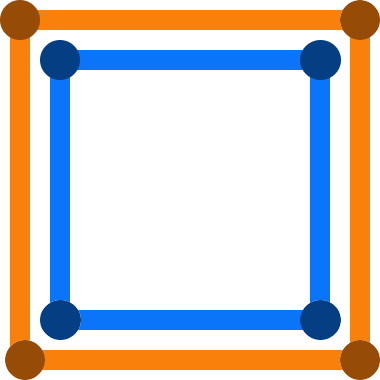
\includegraphics[scale=0.3]{DoubleCage}
  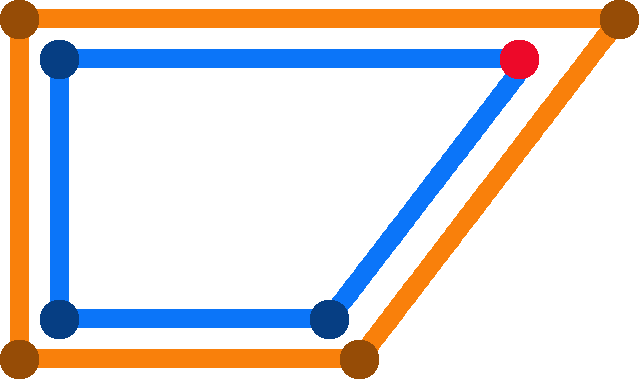
\includegraphics[scale=0.3]{DoubleCage-Hierarchie}
  \caption{Modification de la position du sommet de la cage d'influence associé
  au sommet de la cage de contrôle déplacé (en rouge).}
\end{center}
\end{figure}

\subsubsection{Atténuation de la déformation}

Pour l'instant, la déformation souffre toujours de problème de continuité au
niveau du bord de la cage d'influence. Pour corriger ce problème, nous allons
progressivement atténuer la déformation appliquée, en fonction de la distance
d'un point de l'espace au bord de la cage d'influence.

On souhaite évaluer la distance d'un point de l'espace au bord de la cage
d'influence. On pourrait le faire avec des calculs de distance, mais ça
demanderait de réaliser des opérations supplémentaires. A la place, nous
allons utiliser les coordonnées que nous avons déjà calculé pour chacun des
points de l'espace par rapport aux sommets de la cage d'influence. On définit
donc la distance au bord comme étant égale au produit des poids associés à
chacune des arêtes de la cage d'influence. Où le poids associé à une arête
correspond à la somme des poids associés aux sommets incidents à l'arête
considérée :

\begin{equation}
  d_{inf}(p) = \prod_{e_i \in c_{inf}} (1 - \sum_{v_j \in e_i} \lambda_j)
\end{equation}

Les valeurs de $d_{inf}$ varient entre 0 (bord de la cage d'influence) et
$\frac{2}{n}^n$ (centre de gravité du polygone) où $n$ correspond au nombre de
sommets de la cage d'influence.

Ce calcul s'inspire de la notion de "boundary weight function" de
\cite{GPCP13}, où les auteurs utilisaient cette fonction pour évaluer la
distance d'un point à chacune des arêtes d'une cage.

Nous cherchons maintenant une fonction $f_h(x)$, paramétrée par $h \in ]0,
1]$, permettant de lisser les valeurs des distances des points de l'espace au
bord de la cage d'influence. Cette fonction doit satisfaire $f_h(0) = f_h'(0)
= f_h'(1) = 0$, $f_h(x)=1$ pour $x \geq h$ et $f'_h(x) \geq 0$. L'idée de
cette fonction vient du travail de \cite{GPCP13}, où ils utilisaient cette
fonction pour lisser les valeurs de distance d'un point à une arête de la
cage. Les auteurs proposaient plusieurs fonctions avec des comportements
similaires, nous en avons donc gardé une arbitrairement :

\begin{equation}
  f_h(x) = \frac{1}{2} sin(\pi(\frac{x}{h} - \frac{1}{2})) + \frac{1}{2}
\end{equation}

Il faut définir maintenant la valeur de $h$ afin que ce paramètre représente
la différence de taille entre la cage de contrôle et la cage d'influence. On
souhaite que la déformation ne soit pas atténuée pour l'ensemble des points de
l'espace à l'intérieur de la cage de contrôle. On va donc définir une distance
$d_{min}$ telle que si la distance d'un point de l'espace au bord de la cage
d'influence est supérieure à $d_{min}$, alors la déformation de ce point ne
sera pas atténuée. $d_{min}$ correspond à la plus courte distance d'un point
de l'espace au bord de la cage d'influence. Plus précisément, il s'agit
exactement de la valeur de distance du sommet de la cage de contrôle le plus
proche du bord de la cage d'influence. Il nous suffit donc d'évaluer la valeur
de distance en chacun des sommets de la cage de contrôle par rapport au bord
de la cage d'influence et de les comparer afin de trouver la distance
minimale.

\begin{figure}[ht]
  \begin{center}
    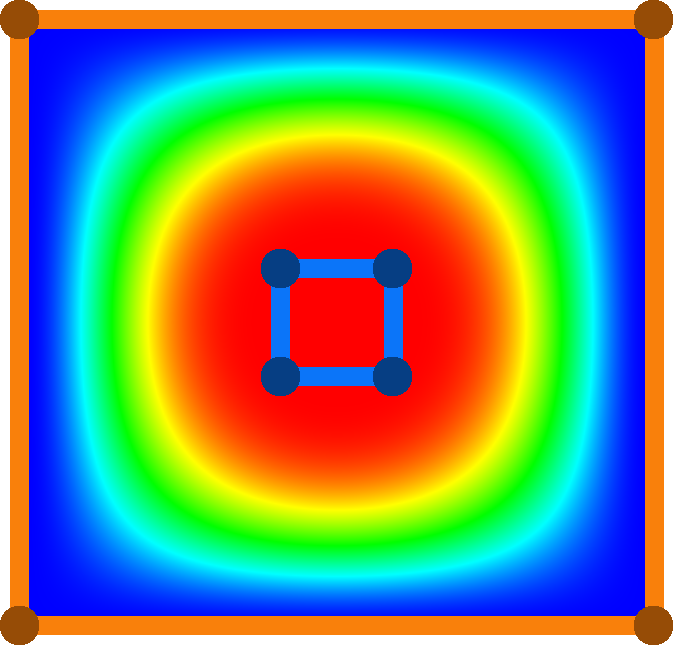
\includegraphics[scale=0.2]{BoundaryWeightFunction-Petite}
    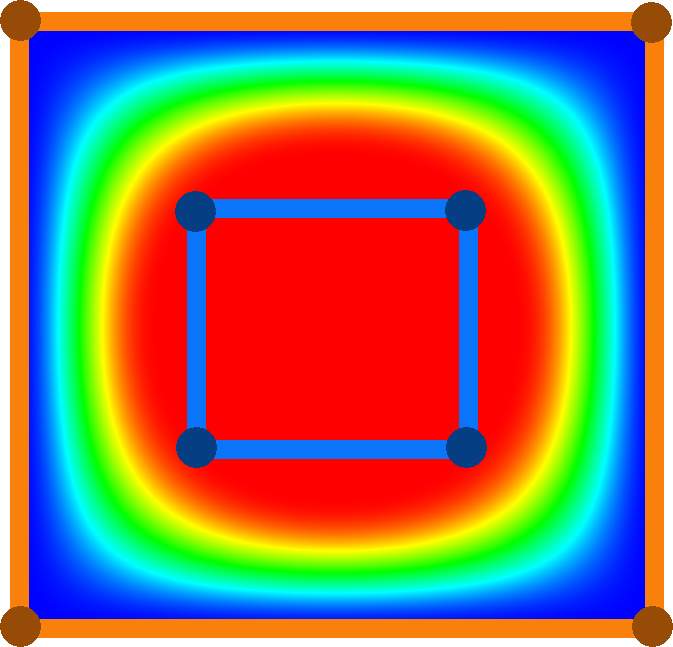
\includegraphics[scale=0.2]{BoundaryWeightFunction}
    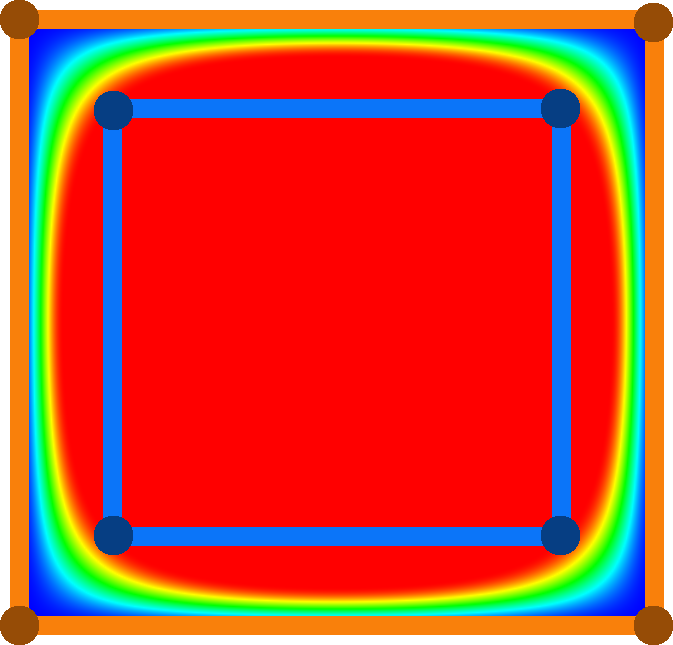
\includegraphics[scale=0.2]{BoundaryWeightFunction-Grande}

    \caption{Variation de l'atténuation de la déformation. La couleur varie du
rouge (atténuation nulle) au bleu (atténuation totale). De gauche à droite on
peut voir la variation pour différentes tailles de cage de contrôle.}

    \label{MELBou}
  \end{center}
\end{figure}

Pour simplifier les écritures dans la suite du travail, nous nous réfèrerons à
ce nouvel outil comme étant l'outil \textit{cage de contrôle d'influence} ou
\textit{cage coninf}.

\subsection{Combinaison des déformations}

Maintenant que nous avons établi un outil de déformation local, nous aimerions
combiner plusieurs cages coninf sur un même objet. L'objectif de cette partie
consiste à trouver une formule de mélange permettant la modification de la
position d'un point de l'espace par rapport à plusieurs cages coninf.

Un point de l'espace aura autant de coordonnées que de cages coninf dans
lesquelles il se situe.

